% Classe du document
\documentclass[aspectratio=169]{beamer}  % Format 16:9 pour un affichage moderne

% Thème et couleurs
\usetheme{Madrid}
\usecolortheme{whale}
\useinnertheme{rectangles}
\useoutertheme{miniframes}
\setbeamertemplate{navigation symbols}{}  % Supprime les symboles de navigation

% Packages essentiels
\usepackage[utf8]{inputenc}
\usepackage[T1]{fontenc}
\usepackage[french]{babel}
\usepackage{lmodern}
\usepackage{amsmath,amssymb,amsthm}
\usepackage{graphicx}
\usepackage{pgfplots}
\usepackage{listings}  % Pour le code
\pgfplotsset{compat=1.18}

% Informations du document
\title[Impact des nouvelles sur les LOB]{Impact des nouvelles sur les \textit{Limit Order Books}}
\subtitle{Une analyse par le modèle Queue-Reactive}
\author[LAFERTE \& AIAD]{LAFERTE Edouard \and AIAD Janis}
\institute[École Polytechnique]{
    Département de mathématiques appliquées\\
    École Polytechnique
}
\date{Juin 2024}

\begin{document}

% Page de titre
\begin{frame}
    \titlepage
\end{frame}







\begin{frame}{Les marchés haute fréquence}
    \begin{itemize}
        \item Électronification des marchés financiers
        \item Réduction drastique du temps d'exécution
        \item Trois catégories de trading:
        \begin{itemize}
            \item \textbf{Low Frequency (LF)}: Échelle de plusieurs mois
            \item \textbf{Mid Frequency (MF)}: Échelle journalière
            \item \textbf{High Frequency (HF)}: Échelle microseconde
        \end{itemize}
    \end{itemize}
\end{frame}


\begin{frame}{Modélisation}
    \begin{itemize}
        \item Mouvement Browninen 
        \item Modèle de jump de Merton
        \item Processus de Hawks
        \item Marche aléatoire du prix sur l'ensemble des tick
        \item Modèle d'agents
        \item Files d'attente
    \end{itemize}
\end{frame}


\begin{frame}{Études empiriques}
    \begin{columns}
        \begin{column}{0.6\textwidth}
            \textbf{Impact des annonces sur le marché}
            \begin{itemize}
                \item \textbf{Volatilité}:
                \begin{itemize}
                    \item Augmentation de 150-300\%
                    \item Pics lors des annonces majeures
                \end{itemize}
                \item \textbf{Liquidité}:
                \begin{itemize}
                    \item Modification des spreads bid-ask
                    \item Changements de profondeur du LOB
                \end{itemize}
            \end{itemize}
        \end{column}
        \begin{column}{0.4\textwidth}
            \begin{alertblock}{Source}
                \small{Review of Financial Studies (2019)}
                \begin{itemize}
                    \item Étude sur impact des news
                    \item Analyse haute fréquence
                    \item Données multi-marchés
                \end{itemize}
            \end{alertblock}
        \end{column}
    \end{columns}
\end{frame}

\begin{frame}{Comportement des Traders et Microstructure}
    \begin{columns}
        \begin{column}{0.6\textwidth}
            \textbf{Déroulé d'une annonce}
            \begin{itemize}
                \item \textbf{Pré-annonce}:
                \begin{itemize}
                    \item Ordres limites prudents
                    \item Positionnement stratégique
                    \item Réduction de l'exposition
                \end{itemize}
                \item \textbf{Post-annonce}:
                \begin{itemize}
                    \item Ordres marchés agressifs
                    \item Exploitation de l'information
                    \item Augmentation de la volatilité
                \end{itemize}
            \end{itemize}
        \end{column}
        \begin{column}{0.4\textwidth}
            \begin{alertblock}{Impact sur le LOB}
                \begin{itemize}
                    \item Volatilité +150-300\%
                    \item Modification des spreads
                    \item Changement de profondeur
                \end{itemize}
            \end{alertblock}
        \end{column}
    \end{columns}
\end{frame}

\begin{frame}{Imbalance et Prédiction}
    \begin{columns}
        \begin{column}{0.6\textwidth}
            \textbf{Mesure d'imbalance}
            \begin{equation*}
                \text{Imb}_t = \frac{Q^{best\ bid}_t-Q^{best\ ask}_t}{Q^{best\ bid}_t+Q^{best\ ask}_t}
            \end{equation*}
            \begin{itemize}
                \item \textbf{Pouvoir prédictif}:
                \begin{itemize}
                    \item Indicateur avancé des prix
                    \item Forte corrélation avec mouvements
                    \item Efficace sur spread 1 tick
                \end{itemize}
            \end{itemize}
        \end{column}
        \begin{column}{0.4\textwidth}
            \begin{alertblock}{Choix des actifs}
                \begin{itemize}
                    \item Focus spread 1 tick
                    \item Réduction du bruit
                    \item Meilleure prédictibilité
                \end{itemize}
            \end{alertblock}
        \end{column}
    \end{columns}
\end{frame}

\begin{frame}{Imbalance}
    \begin{columns}
        \begin{column}{0.48\textwidth}
            \begin{figure}
                \centering
                \includegraphics[width=\textwidth]{Imbalance.png}
                \caption{Imbalance en fonction du $\delta$ tick}
            \end{figure}
        \end{column}
        \begin{column}{0.48\textwidth}
            \begin{figure}
                \centering
                \includegraphics[width=\textwidth]{densité_Imbalance.png}
                \caption{Courbe de distribution de l'imbalance}
            \end{figure}
        \end{column}
    \end{columns}
\end{frame}

\begin{frame}{Problématique}
    \begin{itemize}
        \item Détection d'événements rares sur les marchés financiers
        \item Modélisation des mouvements de prix
        \item Prédiction des sauts de prix
    \end{itemize}
\end{frame}


% Plan
\begin{frame}{Plan de la présentation}
    \tableofcontents
\end{frame}

% Section 1: Introduction aux Limit Order Books
\section{Introduction aux LOB}
\begin{frame}{LOB}
    \begin{columns}[onlytextwidth,totalwidth=\textwidth,columnsep=1em]
        \begin{column}{0.55\textwidth}
            \begin{itemize}
                \item Trois types d'ordres:
                \begin{itemize}
                    \item \textbf{Limit Order}: Proposition à prix fixé
                    \item \textbf{Market Order}: Exécution immédiate
                    \item \textbf{Cancellation}: Retrait d'ordre
                \end{itemize}
                \item Organisation en files d'attente
                \item Prix de référence $p_{ref}$
            \end{itemize}
        \end{column}
        \begin{column}{0.45\textwidth}
            \begin{figure}
                \centering
                \includegraphics[width=0.8\textwidth]{lob.png}
                \caption{Structure d'un Limit Order Book}
            \end{figure}
        \end{column}
    \end{columns}
\end{frame}

% Section 2: Le modèle Queue-Reactive
\section{Le modèle Queue-Reactive}

\begin{frame}{Principes du modèle QR}
    \begin{itemize}
        \item Modélisation par files d'attente
        \item Prix fixe de référence $p_{ref}$
        \item Évolution selon processus de Markov
        \item Variables de Poisson indépendantes
    \end{itemize}
\end{frame}




\begin{frame}{Dynamique du modèle QR}
    \begin{columns}
        \begin{column}{0.6\textwidth}
            \begin{equation*}
                Q(t) = (Q_{-K}(t),...Q_{-1}(t),Q_{1}(t),...Q_K(t))
            \end{equation*}
            \begin{equation*}
                (i_{min}, U_{min}) = \argmin_{(i,U)\in\{-K,K\}\times\{A,C,T\}} \mathcal{P}(\lambda_i^U(Q_i(t)))
            \end{equation*}
            \begin{itemize}
                \item Processus de Poisson d'intensités $\lambda_i^U(Q_i(t))$
                \item $U \in \{\text{Add}, \text{Cancel}, \text{Trade}\}$
                \item \textbf{Mean-reversion double}:
                \begin{itemize}
                    \item $\theta$: retour au prix de référence
                    \item $\theta_{\text{reinit}}$: nouveau $p_{\text{ref}}$ avec LOB invariant
                \end{itemize}
            \end{itemize}
        \end{column}
        \begin{column}{0.4\textwidth}
            \begin{alertblock}{Mécanismes de stabilisation}
                \begin{itemize}
                    \item $\theta$: stabilisation locale
                    \item $\theta_{\text{reinit}}$: adaptation globale
                    \item Loi invariante du LOB
                \end{itemize}
            \end{alertblock}
        \end{column}
    \end{columns}
\end{frame}

\begin{frame}{Représentation du modèle QR}
    \begin{figure}
        \centering
        \includegraphics[width=0.8\textwidth]{representation.png}
    \end{figure}
\end{frame}




\begin{frame}{Probabilité de saut $\theta$}
    \begin{columns}
        \begin{column}{0.6\textwidth}
            \begin{figure}
                \centering
                \includegraphics[width=\textwidth]{tickbid.png}
                \caption{Évolution du LOB et tirage des variables de Poisson}
            \end{figure}
        \end{column}
        \begin{column}{0.4\textwidth}
            \begin{alertblock}{Observations clés}
                \begin{itemize}
                    \item Volatilité observée > volatilité QR
                    \item Même avec $\theta=0$, volatilité insuffisante
                    \item Solution: $\theta_{\text{reinit}}\approx0.13$
                \end{itemize}
            \end{alertblock}
        \end{column}
    \end{columns}
\end{frame}











% Section 0: Données et Méthodologie
\section{Données et Méthodologie}

\begin{frame}{Sources des données}
    \begin{itemize}
        \item \textbf{Nasdaq Databento}:
        \begin{itemize}
            \item Données HF nanoseconde
            \item MBO complets (ITCH)
        \end{itemize}
        \item \textbf{Chicago Mercantile Exchange}:
        \begin{itemize}
            \item Large tick assets, moins d'activité, multi-régime (RIOT)
        \end{itemize}
    \end{itemize}
\end{frame}


\begin{frame}{Prétraitement systématique des données}
    \begin{itemize}
        \item \textbf{Pipeline systématique de nettoyage}:
        \begin{itemize}
            \item Filtrage des données aberrantes
            \item Synchronisation temporelle
            \item Reconstruction du carnet d'ordres
        \end{itemize}
        \item \textbf{Hypothèses validées}:
        \begin{itemize}
            \item Indépendance sur périodes sans drift
            \item Validation empirique sur données
            \item Stationnarité des intensités
        \end{itemize}
    \end{itemize}
\end{frame}


\begin{frame}{Caractéristiques des données}
    \begin{table}
    \centering
    \begin{tabular}{|c|c|c|c|c|}
    \hline
    \textbf{Actif} & \textbf{Nb/Jour Actions} & \textbf{Pct Add} & \textbf{Pct Cancel} & \textbf{Pct Order} \\ \hline
    GOOGL & 2.67M & 49.65\% & 46.64\% & 3.70\% \\ \hline
    LCID & 70.7k & 45.69\% & 42.94\% & 11.35\% \\ \hline
    KHC & 203k & 47.75\% & 45.34\% & 6.89\% \\ \hline
    \end{tabular}
    \caption{Statistiques moyennes sur 65 jours (28 juillet - 4 novembre)}
    \end{table}
    \vspace{0.5cm}
    \begin{itemize}
        \item Focus sur deux titres complémentaires:
        \begin{itemize}
            \item \textbf{GOOGL}: Volume élevé (2.67M/jour), tick fin
            \item \textbf{KHC}: Moins de trades (203k/jour), tick plus large
        \end{itemize}
    \end{itemize}
\end{frame}



\section{Analyse empirique du QR}

\begin{frame}{Prix et limites de GOOGL}
    \begin{columns}
        \begin{column}{0.7\textwidth}
            \begin{figure}
                \centering
                \includegraphics[width=0.7\textwidth]{Prix&limit.png}
                \caption{Évolution du prix de GOOGL avec le bid-ask (2024-07-25, 16:02-16:03). Les points noirs sont les trades, les tracés sont les limites -9 à +9}
            \end{figure}
        \end{column}
        \begin{column}{0.3\textwidth}
            \begin{alertblock}{Validation du modèle QR}
                \begin{itemize}
                    \item Mouvements de prix conformes aux prédictions
                    \item Mean-reversion observée
                    \item Sauts de prix cohérents avec $\theta$
                    \item Imbalances prédictives
                \end{itemize}
            \end{alertblock}
        \end{column}
    \end{columns}
\end{frame}

\begin{frame}{Intensité première limite}
    \begin{columns}
        \begin{column}{0.48\textwidth}
            \begin{figure}
                \centering
                \includegraphics[width=\textwidth]{Trades.png}
                \caption{Intensité des trades}
            \end{figure}
        \end{column}
        \begin{column}{0.48\textwidth}
            \begin{figure}
                \centering
                \includegraphics[width=\textwidth]{ADD_Cancel.png}
                \caption{Intensité des Add et des Cancels}
            \end{figure}
        \end{column}
    \end{columns}
\end{frame}

\begin{frame}{Intensitées seconde limite}
            \begin{figure}
                \centering
                \includegraphics[width=0.6\textwidth]{2ndLim_Intensity.png}
                \caption{Intensité des Add et des Cancels}
            \end{figure}

\end{frame}

\begin{frame}{Imbalance}
    \begin{columns}
        \begin{column}{0.48\textwidth}
            \begin{figure}
                \centering
                \includegraphics[width=\textwidth]{KHC_Trades_ints_imb.png}
                \caption{Trades}
            \end{figure}
        \end{column}
        \begin{column}{0.48\textwidth}
            \begin{figure}
                \centering
                \includegraphics[width=\textwidth]{ADD_CANCEL_INTENSITY_IMBALNCE_LCID.png}
                \caption{Add \& Cancels}
            \end{figure}
        \end{column}
    \end{columns}
\end{frame}

\begin{frame}{Cas particulier de RIOT}
    \begin{columns}
        \begin{column}{0.6\textwidth}
            \textbf{Deux régimes distincts observés}:
            \begin{itemize}
                \item \textbf{Régime 1}: Trading classique
                \begin{itemize}
                    \item Dynamique de marché standard
                    \item Variation des prix normale
                \end{itemize}
                \item \textbf{Régime 2}: Trading suspect
                \begin{itemize}
                    \item Prix constants sur longues périodes
                    \item Volumes d'échange importants
                    \item Potentiels accords hors marché
                \end{itemize}
            \end{itemize}
        \end{column}
        \begin{column}{0.4\textwidth}
            \begin{alertblock}{Particularités CME}
                \begin{itemize}
                    \item Transactions répétées au même prix
                    \item Volumes prédéfinis
                    \item Possible entente entre acteurs
                    \item Marché Chicago spécifique
                \end{itemize}
            \end{alertblock}
        \end{column}
    \end{columns}
    \vspace{0.2cm}
    \begin{itemize}
        \item \textbf{Implications}:
        \begin{itemize}
            \item Nécessité de filtrer ces périodes
            \item Biais potentiel dans l'analyse
            \item Question de la manipulation de marché
        \end{itemize}
    \end{itemize}
\end{frame}





\begin{frame}{Régimes de spread sur RIOT}
    \begin{columns}
        \begin{column}{0.6\textwidth}
            \begin{figure}
                \centering
                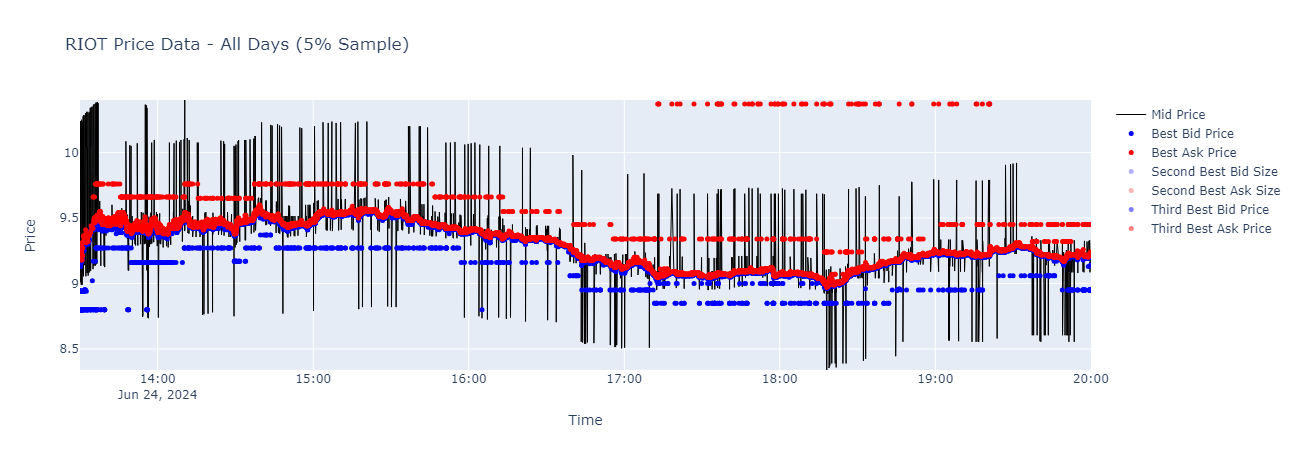
\includegraphics[width=\textwidth]{riot.png}
                \caption{Trois régimes de spread distincts sur RIOT}
            \end{figure}
        \end{column}
        \begin{column}{0.4\textwidth}
            \begin{alertblock}{Régimes observés}
                \begin{itemize}
                    \item \textbf{Régime 1}: Spread minimal
                    \begin{itemize}
                        \item 3 limites actives
                        \item Spread 1 tick
                    \end{itemize}
                    \item \textbf{Régime 2}: Spread intermédiaire
                    \begin{itemize}
                        \item 2 limite active
                        \item Spread 25 ticks
                    \end{itemize}
                    \item \textbf{Régime 3}: Spread large
                    \begin{itemize}
                        \item 1 limite active
                    \end{itemize}
                \end{itemize}
            \end{alertblock}
        \end{column}
    \end{columns}
    \begin{itemize}
        \item \textbf{Transition rapide entre régime}
        \end{itemize}
    \end{itemize}
\end{frame}


% Section 3: Théorèmes principaux
\section{Intensité de news théorique}

\begin{frame}{Notations}
     \hspace{1cm}
    \begin{itemize}
        \item \textbf{Vecteur d'état}$$\eta_t = (\text{Imb}_t, \Delta_t, {A_t}), \ t\in\{t_1,t_2,\dots,t_n\}\in [0,T_f]^n $$
        \item \textbf{Séparation en bucket d'imbalance} $$\mathcal I= \{\mathcal I^1,\dots,\mathcal I^m\}$$
        \item \textbf{Redéfinition par} $$\tilde \eta_t^T = \left(\text{Imb}_t, \frac{\Delta_t}{\sum_{i=1}^m\mu_i^n\mathbb{I}_{\text{Imb}_t\in\mathcal{I}^{i}}}\right), \ \text{avec } \mu_i^n = \frac{1}{\#\{j\in \mathcal I^i\}}\sum_{j\in \mathcal I^i}^n\Delta_{t_i}$$
        \item $\Delta_T^{n_T}(\alpha)$ qui correspond au quantile d'ordre $1-\alpha$ de la famille $\tilde \eta_t^T$
    \end{itemize}
\end{frame}

\begin{frame}{Convergence du quantile}
    \begin{theorem}[Convergence du quantile]
        La valeur $\Delta_T^{n_T}(\alpha)$ tend vers une constante $\Delta_T(\alpha)$ qui ne dépend plus de $T_f$:
        \begin{align*}
            T_f &\underset{n\to +\infty}{\to}+\infty \ \text{p.s} \\
            \frac{n_T}{n} &\underset{n\to +\infty}{\to}C^{ste} \ \text{p.s} \\
            \Delta_T^{n_T}(\alpha) &\underset{n\to +\infty}{\to}\Delta_T(\alpha) \ \text{p.s}
        \end{align*}
    \end{theorem}
\end{frame}



\section{Analyse empirique des news}


\begin{frame}{Événements majeurs (1/3)}
    \begin{columns}
        \begin{column}{0.48\textwidth}
            \begin{figure}
                \centering
                \includegraphics[width=\textwidth]{Graphe_1.png}
                \caption{20 sept. 2024: Plainte UK monopole\\
                Impact fort et immédiat sur le LOB}
            \end{figure}
        \end{column}
        \begin{column}{0.48\textwidth}
            \begin{figure}
                \centering
                \includegraphics[width=\textwidth]{Graphe4.png}
                \caption{25 juil. 2024: Résultats Q2 + ChatGPT\\
                Double impact: financier et technologique}
            \end{figure}
        \end{column}
    \end{columns}
\end{frame}

\begin{frame}{Événements majeurs (2/3)}
    \begin{columns}
        \begin{column}{0.48\textwidth}
            \begin{figure}
                \centering
                \includegraphics[width=\textwidth]{Graphe5.png}
                \caption{17 nov. 2024: Gemini + Pixel 9\\
                Impact technologique majeur}
            \end{figure}
        \end{column}
        \begin{column}{0.48\textwidth}
            \begin{figure}
                \centering
                \includegraphics[width=\textwidth]{Graphe6.png}
                \caption{29 août 2024: Faille Chrome\\
                Réaction rapide mais limitée}
            \end{figure}
        \end{column}
    \end{columns}
\end{frame}

\begin{frame}{Événements majeurs (3/3)}
    \begin{columns}
        \begin{column}{0.48\textwidth}
            \begin{figure}
                \centering
                \includegraphics[width=\textwidth]{Graphe7.png}
                \caption{18 sept. 2024: Cut FED\\
                Impact macroéconomique global}
            \end{figure}
        \end{column}
        \begin{column}{0.48\textwidth}
            \begin{figure}
                \centering
                \includegraphics[width=\textwidth]{Grpahe7.png}
                \caption{5 août 2024: Amende US\\
                Impact réglementaire direct}
            \end{figure}
        \end{column}
    \end{columns}
\end{frame}

\begin{frame}{Synthèse des événements majeurs}
    \begin{columns}
        \begin{column}{0.48\textwidth}
            \begin{alertblock}{Caractéristiques communes}
                \begin{itemize}
                    \item Asymétrie des réactions selon nature de la news
                    \item Temps de réaction différents selon l'événement
                    \item Impact sur la profondeur du carnet
                    \item Réaction instantanée du marché
                    \item Modification profonde de la structure du LOB
                    \item Persistance des effets sur plusieurs minutes
                \end{itemize}
            \end{alertblock}
        \end{column}
        \begin{column}{0.48\textwidth}
            \begin{alertblock}{Synthèse des impacts}
                \begin{itemize}
                    \item Hiérarchie claire des impacts selon type de news
                    \item Patterns de réaction spécifiques
                    \item Corrélation avec volume d'échanges
                    \item Classification possible des événements:
                    \begin{itemize}
                        \item Impacts réglementaires
                        \item Impacts technologiques
                        \item Impacts macroéconomiques
                    \end{itemize}
                \end{itemize}
            \end{alertblock}
        \end{column}
    \end{columns}
\end{frame}

\begin{frame}{Impact des news sur la microstructure}
            \begin{figure}
                \centering
                \includegraphics[width=0.8\textwidth]{newploit.png}
                \caption{18 sept. 2024: Cut FED\\
                Impact macroéconomique global}
            \end{figure}
\end{frame}

% Remerciements
\begin{frame}{Remerciements}
    \begin{center}
        \Large Merci de votre attention
        \vspace{1cm}
        
        \normalsize
        Questions?
    \end{center}
\end{frame}

\end{document}